\documentclass[12pt]{article}
\usepackage{tikz}
\usepackage{amssymb}
\usepackage{amsmath}
\usepackage{breqn}

\usetikzlibrary{automata, positioning, arrows}

\title{SE 3310 Theoretical Foundations of Software Engineering Assignment 1}
\author{Marcus Tuen Muk}
\date{January 26 2023}


\begin{document}

    \begin{titlepage}
        \clearpage\maketitle
        \thispagestyle{empty}
    \end{titlepage}

    \section{Identify the regular languages}
        \subsection{\[L_a = \{wwwa^n:w \in \{a,b\}, n > 0\}\]}
            \indent
            Based on this language, w is either all a or all b. This language is a regular language.
            \begin{figure}[ht]
                \centering
                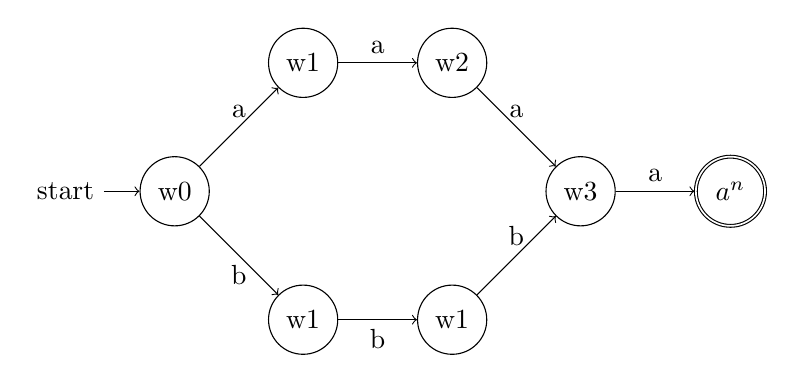
\begin{tikzpicture}
                    \node[state, initial] (w0) {w0};
                    \node[state, above right = of w0] (a1) {w1};
                    \node[state, right = of a1] (a2) {w2};
                    \node[state, below right =of w0] (b1) {w1};
                    \node[state, right =of b1] (b2) {w1};
                    \node[state, below right =of a2] (w3) {w3};
                    \node[state, accepting, right =of w3] (an) {\(a^n\)};
                    

                    \draw   (w0) edge[->, right, above] node{a} (a1)
                            (w0) edge[->, right, below] node{b} (b1)
                            (a1) edge[->, right] node[above] {a} (a2)
                            (b1) edge[->, right] node[below] {b} (b2)
                            (a2) edge[->, right] node[above] {a} (w3)
                            (b2) edge[->, right] node[above] {b} (w3)
                            (w3) edge[->, right] node[above] {a} (an);
                        
                \end{tikzpicture}  
            \end{figure}
        
            \pagebreak
            
            \subsection{\[L_b = \{w \in \{0,1\}*:w \ represents \ as \ a \ binary \ integer \ is \ a \ power \ of \ 4\}\]}
                \indent
                This language is a regular language.
                \begin{figure}[ht]
                    \centering
                    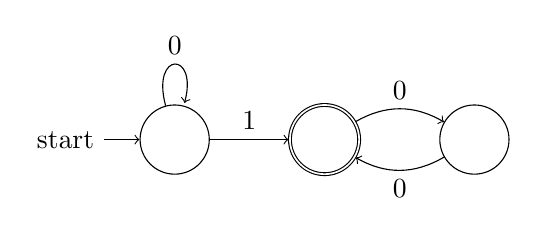
\begin{tikzpicture}
                        \node[state, initial] (w0) {};
                        \node[state, accepting, right = of w0] (w1) {};
                        \node[state, right = of w1] (w2) {};

                        \draw   (w0) edge[->, loop above] node{0} (w0)
                                (w0) edge[->, right] node[above] {1} (w1)
                                (w1) edge[->, bend left] node[above] {0} (w2)
                                (w2) edge[->, bend left] node[below] {0} (w1);
                            
                    \end{tikzpicture}  
                \end{figure}

                \pagebreak

                \subsection{\[L_c = \{wxa: w,x \in \{a,b\}*\}\]}
                \indent
                This language is a regular language.
                \begin{figure}[ht]
                    \centering
                    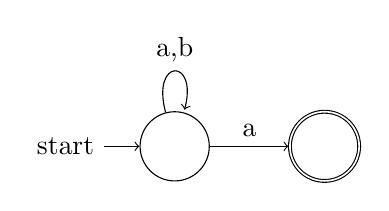
\begin{tikzpicture}
                        \node[state, initial] (wx0) {};
                        \node[state, accepting, right = of wx0] (a) {};

                        \draw   (wx0) edge[->, loop above] node{a,b} (wx0)
                                (wx0) edge[->, right] node[above] {a} (a);
                            
                    \end{tikzpicture}  
                \end{figure}

                \pagebreak

                \subsection{\[L_c = \{wwa: w,x \in \{a,b\}*\}\]}
                \indent
                This language is not a regular language. This language states that some w is a string that
                can be of length 0 or greater and will occur twice. As such, it would need the Finite state
                Machine (FSM) to store the length of w to ensure both strings are the same length. However,
                FSM don't have this capability, thus making this language not a regular language.
                
            \pagebreak 

        \section{Describe the language}
            The formal description of a DFA \emph{M} is given as follows. 
            Let: \[S = \{q_0, q_1, q_2, q_3\}\]
                \[\Sigma = \{a, b, c\}\]
                \[start = q_0\]
                \[F= \{q_3\}\]
            \\ and let $\delta$ be given by the following table:
                \begin{center}
                    \begin{tabular}{ c |c c c}
                         & a & b & c \\ 

                        \hline

                        $q_0$ & $q_1$ & $q_2$ & $q_0$ \\ 
                        $q_1$ & $q_3$ & $q_2$ & $q_2$ \\
                        $q_2$ & $q_1$ & $q_3$ & $q_1$ \\
                        $q_3$ & $q_3$ & $q_3$ & $q_3$ \\  
                    \end{tabular}
                \end{center}
                
            \pagebreak
            \subsection{Give the state diagram of this machine}
                \begin{figure}[ht]
                    \centering
                    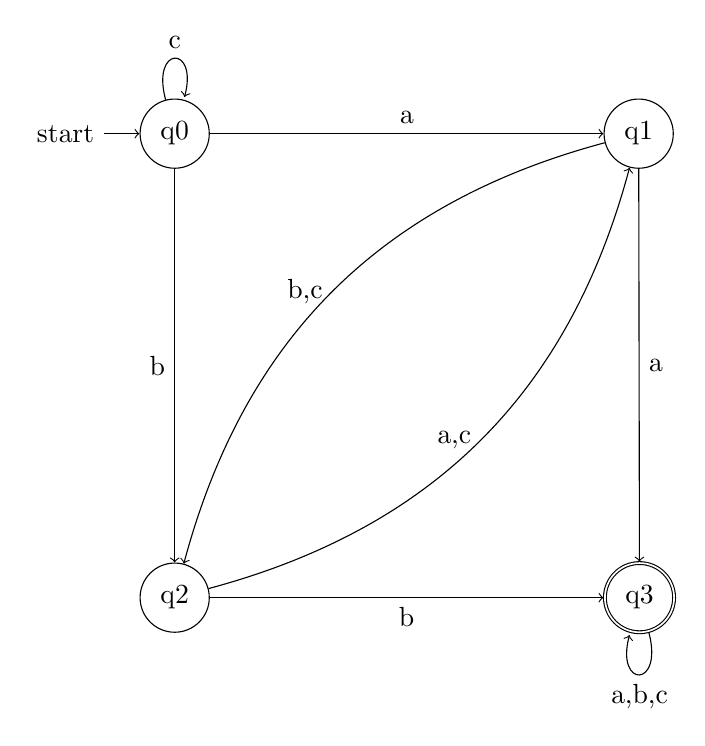
\begin{tikzpicture}
                        \node[state, initial] (q0) {q0};
                        \node[state, right = 5cm of q0] (q1) {q1};
                        \node[state, below = 5cm of q0] (q2) {q2};
                        \node[state, accepting, right = 5cm of q2] (q3) {q3};

                        \draw   (q0) edge[->, loop above] node[above] {c} (q0)
                                (q0) edge[->, right] node[above]{a} (q1)
                                (q0) edge[->, below] node[left] {b} (q2)
                                (q1) edge[->, bend right] node[left] {b,c} (q2)
                                (q2) edge[->, bend right] node[left] {a,c} (q1)
                                (q1) edge[->, below] node[right] {a} (q3)
                                (q2) edge[->, right] node[below] {b} (q3)
                                (q3) edge[->, loop below] node[below] {a,b,c} (q3);
                            
                    \end{tikzpicture}  
                \end{figure}

                \pagebreak

                \subsection{Using \emph{set builder}, discribe the language accepted by \emph{M}}

                    \begin{multline}
                       [L_{M} = \{c^nwxc^myz : n,m \in \mathbb{Z}, n,m \geq 0^*, w,x,y \in \{a,b\}^*, z \in \{a,b,c\}, \\ 
                        if \ m \ is \ even \ then \ x=y, else \ x \neq y\}]
                    \end{multline}

                \pagebreak

            \section{Recognizing decimal integers divisible by 5}
                \subsection{Let string \(s \in \{0, ..., 9\}^*\), \(n\) be string \(s\) interpreted as a decimal integer. Draw a DFA that accepts \(s\) if and only if: \[n \equiv 0 \ mod \ 5\] assume \(\epsilon \not\equiv 0 \ mod \ 5\)}
                
                \begin{figure}[ht]
                    \centering
                    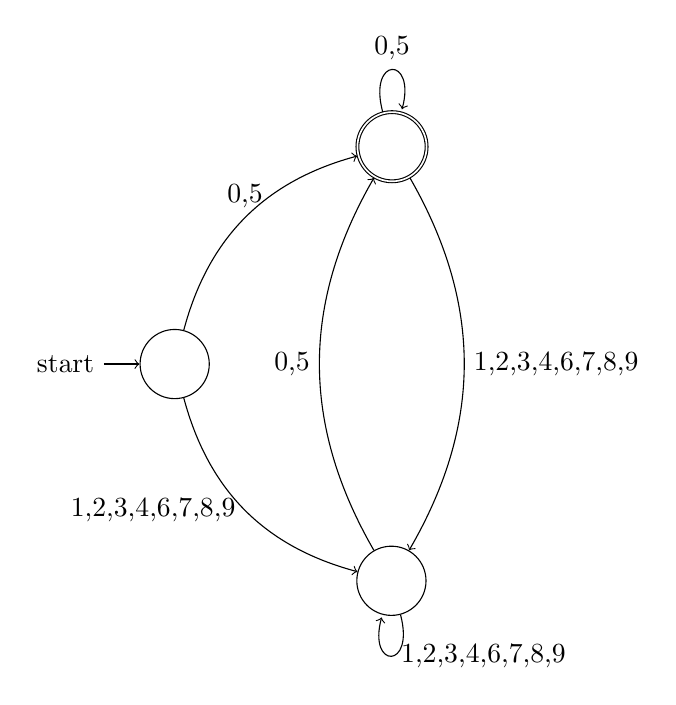
\begin{tikzpicture}
                        \node[state, initial] (q0) {};
                        \node[state, accepting, above right = 3cm of q0] (q1) {};
                        \node[state, below right = 3cm of q0] (q2) {};
                        
                        \draw   
                                (q0) edge[->, bend left] node[above]{0,5} (q1)
                                (q0) edge[->, bend right] node[left] {1,2,3,4,6,7,8,9} (q2)
                                (q1) edge[->, bend left] node[right] {1,2,3,4,6,7,8,9} (q2)
                                (q2) edge[->, bend left] node[left]{0,5} (q1)
                                (q2) edge[->, loop below] node[right] {1,2,3,4,6,7,8,9} (q2)
                                (q1) edge[->, loop above] node[above]{0,5} (q1);
                    \end{tikzpicture}  
                \end{figure}    

            \pagebreak
            \section{Design NFAs}
                Let \(\Sigma = \{a,b,c\}\). Draw an NFA recognizing each of the following languages:  
                
                \subsection{The set of strings that contain c's in runs of no more than two (e.g., a, ac, acc, etc. but not strings like accc, acccc, etc.)}
                    \begin{figure}[ht]
                            \centering
                            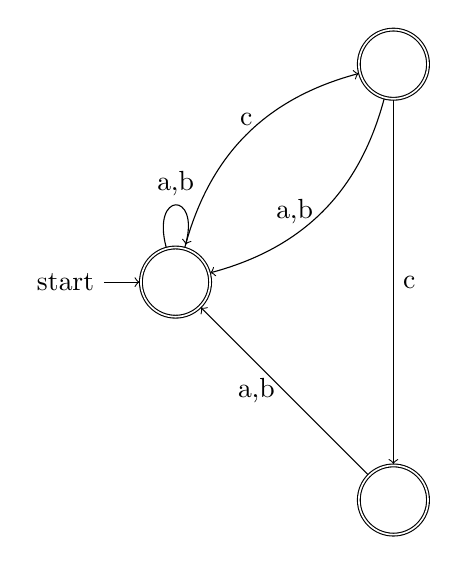
\begin{tikzpicture}
                                \node[state, accepting, initial] (q0) {};
                                \node[state, accepting, above right = 3cm of q0] (q1) {};
                                \node[state, accepting, below right = 3cm of q0] (q2) {};
                                
                                \draw   
                                        (q0) edge[->, loop above] node[above]{a,b} (q0)
                                        (q0) edge[->, bend left] node[above]{c} (q1)
                                        (q1) edge[->, bend left] node[left]{a,b} (q0)
                                        (q2) edge[->, right] node[left] {a,b} (q0)
                                        (q1) edge[->,  left] node[right] {c} (q2);
                            \end{tikzpicture}  
                        \end{figure}  
            
                \pagebreak
                \subsection{The set of strings that contain no consecutive letters (e.g., a 'b' cannot follow a 'b').}
                    \begin{figure}[ht]
                            \centering
                            \begin{tikzpicture}
                                \node[state, accepting, initial] (q0) {};
                                \node[state, accepting, above right = 8cm of q0] (q1) {};
                                \node[state, accepting, right = 1cm of q0] (q2) {};
                                \node[state, accepting, below right = 8cm of q0] (q3) {};
                                
                                \draw   
                                        (q0) edge[->, bend left] node[above]{a} (q1)
                                        (q0) edge[->, right] node[above]{b} (q2)
                                        (q0) edge[->, bend right] node[below]{c} (q3)
                                        (q2) edge[->, right] node[left]{a} (q1)
                                        (q3) edge[->, above] node[right]{a} (q1)
                                        (q1) edge[->,  bend right] node[left]{b} (q2)
                                        (q3) edge[->, bend right] node[right]{b} (q2)
                                        (q1) edge[->,  bend left] node[left]{c} (q3)
                                        (q2) edge[->, right] node[right]{c} (q3);
                                        
                            \end{tikzpicture}  
                        \end{figure} 
                
\end{document}